\section{Supplementary Methods}
\subsection{Demographic correction}

DFE-alpha corrects for population demographic history when inferring selection parameters. However, there are several processes that can cause distortions of the uSFS that are not captured using the relatively simple demographic models. In particular, we found that the high frequency elements of the uSFS are not accurately captured under the demographic models implemented in DFE-alpha (Figure S1) (see main text). We make the assumption that the processes causing distortions to the uSFS for neutral sites also affect the selected site uSFS. Under this assumption, we correct the individual elements of the uSFS for selected sites using Equation 7 from \cite{RN321}:

\begin{equation}
N`_j = \frac{N_j}{1 + \frac{S_j - E_j}{E_j}} for j = 0,1,2 ... n
\end{equation}

Where $N_j$ is the number of derived mutations present in $j$ copies in the selected site data and $S_j$ and $E_j$ are the observed and expected number of mutations at frequency $j$ in the synonymous site data. Expected numbers of sites come from the fit of a neutral demographic model. Conceptually similar corrections have been applied by \cite{RN354,RN276,RN275}.

\subsection{Divergence correction}

Likelihoods in DFE-alpha are calculated using the allele frequency vector (AFV). The AFV is a vector of counts for mutations at different frequencies, accounting for population size change and selection. In a sample of alleles drawn from a population, polymorphic sites may resemble fixed derived mutations due to sampling effects. For each element of the AFV, we calculate the binomial probability of observing 20 fixed derived alleles (the number of samples in the \textit{M. m. castaneus} data). The expected proportion of spurious fixed derived sites is then subtracted from the observed data and re-distributed to the polymorphic bin using the AFV to apportion out the number of sites appropriately.

We implemented the divergence correction in an iterative fashion as follows. After fitting demographic models or selection models to the uSFS using DFE-alpha, we remove the number of sites from the fixed derived class of sites and redistribute the proportion removed to polymorphism bins using the AFS estimated from the model fitted as described above. The resulting uSFS is then fitted using DFE-alpha as before. This procedure is repeated until the likelihood difference between successive iterations is less than 1.0. In all cases of applying this correction, likelihoods converged within 5 iterations.

\subsection{Ancestral effective population size, Ne-anc – Model B}

Between-species divergence and within-species polymorphism may not reflect the same suite of processes. If, for example, in the time since a focal species split from the outgroup used to estimate the uSFS the DFE for advantageous mutations changed, the between-species divergence at selected sites will reflect a combination of the current DFE and the previous one. Polymorphisms present in the population at the time of sampling, however, may only reflect the most recent DFE. This is because divergence is accumulated over all time since the split of the focal species and the outgroup while polymorphism may only reflect recent processes. If polymorphism and divergence have become decoupled including fixed derived sites when estimating selection parameters may lead to bias. Indeed,  \cite{RN354} showed that accurate estimates of selection parameters can be obtained solely from the polymorphism data in the uSFS. 

We modified the likelihood function of \cite{RN210} by adding an additional parameter, that we call the ancestral effective population size ($N_{e-anc}$ ). $N_{e-anc}$  is fitted solely to the fixed derived class of sites. Fitting $N_{e-anc}$  has the effect of absorbing the contribution of fixed derived sites, so that selection parameters are estimated from polymorphism and invariant ancestral sites only. We define $N_{e-anc}$ size as the population size that, given the current estimates of the selection coefficients, satisfies the number of fixed derived mutations in the sample. We use Kimura’s formula for the fixation probability ($Q$) of a selected allele in a population of size $N$:

\begin{equation}
Q = \frac{(1 - e^{-s_a})}{1-e^{-2N_es_a}}
\end{equation}
where $s$ is the selection coefficient for homozygotes, and $N_e$ is the effective population size. Models that do not incorporate $N_{e-anc}$ are nested within those that do, so likelihood ratio tests can be used for comparisons. Model B in the main text fits the $N_{e-anc}$ parameter alongside the selection parameters. Because polymorphism and divergence could potentially become decoupled by multiple processes, the value of $N_{e-anc}$ is difficult to interpret. 

\section{Supplementary Tables and Figures}

\begin{sidewaystable}
\caption[Summary of recombination rates per chromosomes]{Summary of sex-averaged recombination rates \emph{M. m castaneus} compared with the rates from Brunschwig et al. (2012) and Cox et al. (2009). Rates for the castaneus and Brunschwig maps are presented in terms of $4N_{e}r/bp$. Estimates of $N_e$ were obtained by assuming the recombination rates from Cox et al. (2009).}
 \begin{tabular}{c c c c c c c c c } 
  \hline
& & &  & & \multicolumn{3}{c}{Switch Errors} &  \\
Filter Set & HWE & Min DP & Max DP & Min GQ & H40 & H46 & H62 & \\ \hline
1 & - & - & - & - & 5,148/409,486 & 4,819/407,422 & 5,020/394,778 & 0.0124 \\
2 & <0.0002 & 10 & - & 15 & 1,690/338,592 & 1,451/334,111 & 1,452/324,199 & 0.0046 \\
3 & <0.0002 & 10 & 100 & 5 & 2,460 /341,744 & 2066 /339,508 & 2536 /328,998 & 0.0070 \\
4 & <0.0002 & - & - & 40 & 523 /288,471 & 444 /286,636 & 550 /281,266 & 0.0018 \\
 \hline
\end{tabular}    
 \label{tab:C2ST1}
\end{sidewaystable}

	

\begin{table}[h!]
\centering
\caption[Parameters of the best-fitting demographic model estimated from the analysis of 4-fold and CNE-flanking sites]{Parameters of the best-fitting demographic model estimated from the analysis of 4-fold and CNE-flanking sites. }
 \begin{tabular}{c c c c c } 

\toprule
	&4-fold	&CNE-flank \\ \hline
N2/N1&	0.40&	0.07 \\
t2/N1&	0.44&	0.17 \\
N3/N1&	0.40&	1.00 \\
t3/N1&	1.10&	0.63 \\
\bottomrule

\end{tabular}
\label{tab:CS2}
\end{table}

\begin{table}[h!]
\centering
\caption[Parameters of the 3-epoch demographic model at different sample sizes]{Parameters of the 3-epoch demographic model at different sample sizes. Down sampled datasets were generated by randomly selecting alleles, with respect to frequency, from the full dataset of 10 individuals.}
 \begin{tabular}{c c c c c } 

\toprule
\multirow{2}{*}{Parameter} & \multicolumn{3}{c}{Number of alleles sampled} \\ 
	&	$n = 10$ & 	$n = 16$ & 	$n = 20$ \\ \hline
N2/N1 &	0.030 &	0.030 &	0.060 \\
t2/N1 &	0.204 &	0.140 &	0.181 \\
N3/N1 &	0.120 &	0.200 &	0.800 \\
t3/N1 &	0.080 &	0.220 &	0.461 \\
\bottomrule

\end{tabular}
\label{tab:CS3}
\end{table}



\begin{table}
\caption{The overlap between the hotspots we identified in M. m. castaneus and the locations of DSB hotspots in wild-derived strains obtained by Smagulova et al. (2016). The corrected overlap is the number of overlapping hotspots, above the null expectation, over the total.}
\begin{tabular} {c c c c c c c} \\ [ 0.5ex ] \hline

\makecell{Strain\\ID} & Sub-species & \makecell{\# DSB \\ Hotspots} & \makecell{\# \\ Overlaps} & \makecell{\% Overlap \\ Uncorrected} & \makecell{Null \\Expectation} & \makecell{\% Overlap \\ Corrected}\\ \hline
13R & \emph{domesticus} & 14744 & 1202 & 8.2 & 1169 & 0.2 \\
B6 & \emph{domesticus}& 19455 & 1533 & 7.9 & 1505 & 0.1 \\ 
C3H & \emph{domesticus} & 14635 & 1399 & 9.6 & 1308 & 0.6 \\
CAST & \emph{castaneus} & 15061 & 1831 & 12.2 & 1221 & 4.1 \\
MOL & \emph{molossinus} & 15718 & 1559 & 9.9 & 1351 & 1.3 \\
PWD & \emph{musculus} & 14483 & 1569 & 10.8 & 1205 & 2.5 \\ \hline


\end{tabular}
\end{table}


\begin{table}[h!]
\centering
\caption[Parameter estimates for the scaled effect and frequency of advantageous mutations in three classes sites]{Parameter estimates for the scaled effect and frequency of advantageous mutations in three classes sites in \textit{Mus musculus castaneus} when models incorporated either one class of advantageous mutations, or two. }
 \begin{tabular}{c c c c c c c} 
\toprule
\multirow{2}{*}{\textbf{\# Adv. Mutation Classes}} &	\multicolumn{2}{c}{\textbf{0-fold}}	& \multicolumn{2}{c}{\textbf{UTR}}	& \multicolumn{2}{c}{CNE\textbf{}} \\ \cline{2-7}
	& \textbf{1} &	\textbf{2} &	\textbf{1} &	\textbf{2} &\textbf{	1} &\textbf{	2} \\ \hline 
 &	\multicolumn{6}{c}{\textbf{Model A: Full uSFS}} \\ \hline
$N_es_{a,1}$	 & 7.27	& 7.27	& 5.32	& 5.32	 & 9.17	 & 9.17 \\
$p_{a,1}$ &	0.003	& 0.003	& 0.0133 & 	0.0133 &	0.0098 &	0.0098 \\
$N_es_{a,2}$ & 	- &	0.000 &	- &	0.000 &	- &	0.000 \\
$p_{a,2}$ &	-	& 0.000	& -	& 0.000 &	- &	0.000 \\
$\Delta lnL$ &	-	 & 0.000 &	-	& 0.005	& - &	0.000 \\ \hline
 &	\multicolumn{6}{c}{\textbf{Model B: Ignoring sites fixed for the derived allele}} \\ \hline
$N_es_{a,1}$ &	8.30	 & 8.30	& 6.96	& 6.96	& 8.60	& 8.60 \\
$p_{a,1}$ &	0.010 &	0.010	& 0.0294 &	0.0294	& 0.008 &	0.008 \\
$N_es_{a,2}$ &	- &	0.0925 &	- &	33.6	 & - &	0.240 \\
$p_{a,2}$ &	- &	0.000 &	- &	0.000 &	- &	0.000 \\
$\Delta lnL$  &	- &	0.000 &	- &	0.000 	& - &	0.002 \\
\bottomrule
\end{tabular}
\label{tab:CS5}
\end{table}

\begin{table}[h!]
\centering
\caption[Parameters of the selection and demographic models when estimated from simulated data]{Parameters of the selection and demographic models when estimated from simulated data. The upper portion of the table shows the selection parameters. The selection model simulated contained two classes of deleterious mutational effects and a single class of advantageous mutations. The lower portion of the table contains the demographic parameters inferred for \textit{M. m. castaneus} compared with those inferred from simulation data.}
 \begin{tabular}{c c c c c c c} 
 \toprule
	& & 	\multicolumn{2}{c}{\textbf{Model A}}	& \multicolumn{2}{c}{\textbf{Model B}}   \\ 
	& &	Simulated &	Estimated	& Simulated &	Estimated \\ \hline
	&$N_es_0$ &	-0.045	&-0.70 &	-0.171 & 	-0.40 \\
	&$p_0$ &	 0.191	& 0.145	& 0.184	& 0.181 \\
	&$N_es_1$ &	-104	&-92.3&	-100 &	-77.3 \\
	&$p_1$ &	 0.806	&0.784	& 0.806 &	0.799 \\
	&$N_es_a$ & 	7.27	 & 0.950 &	8.30 &	4.91 \\
	&$p_a$ &	 0.00300	&0.0710&	0.0100&	0.0200 \\ \hline
	& \textit{M. m. castaneus} & & & \\ \hline
$N2/N1$	& 0.40	&-	&0.20&	-	&0.12 \\
$N3/N1$	& 1.4	&-	&1.0	&-	&0.9\\
$t2/N2$	& 0.31	&-	&0.46&	-&	1.2\\
$t3/N3$	& 0.79	&-	&1.4	&-	&1.3 \\
\bottomrule

\end{tabular}
\label{tab:C3S6}
\end{table}

\begin{table}[h!]
\centering
\caption[Parameters of strongly selected mutations assumed in simulations]{Parameters of strongly selected mutations assumed in simulations.}
 \begin{tabular}{c c c c c } 

\toprule
$2N_es_a	$ & $p_a$	& $2N_es_ap_a$ \\ \hline
400 &	0.000218	 & 0.0872 \\
400 &	0.000109	 & 0.0436 \\
200 &	0.000436	 & 0.0872 \\
200 &	0.000218	 & 0.0436 \\
100 &	0.000436	 & 0.0436 \\
\bottomrule

\end{tabular}
\label{tab:CS7}
\end{table}


 \begin{figure}[h!]
   \centering      
   \noindent\makebox[\textwidth]{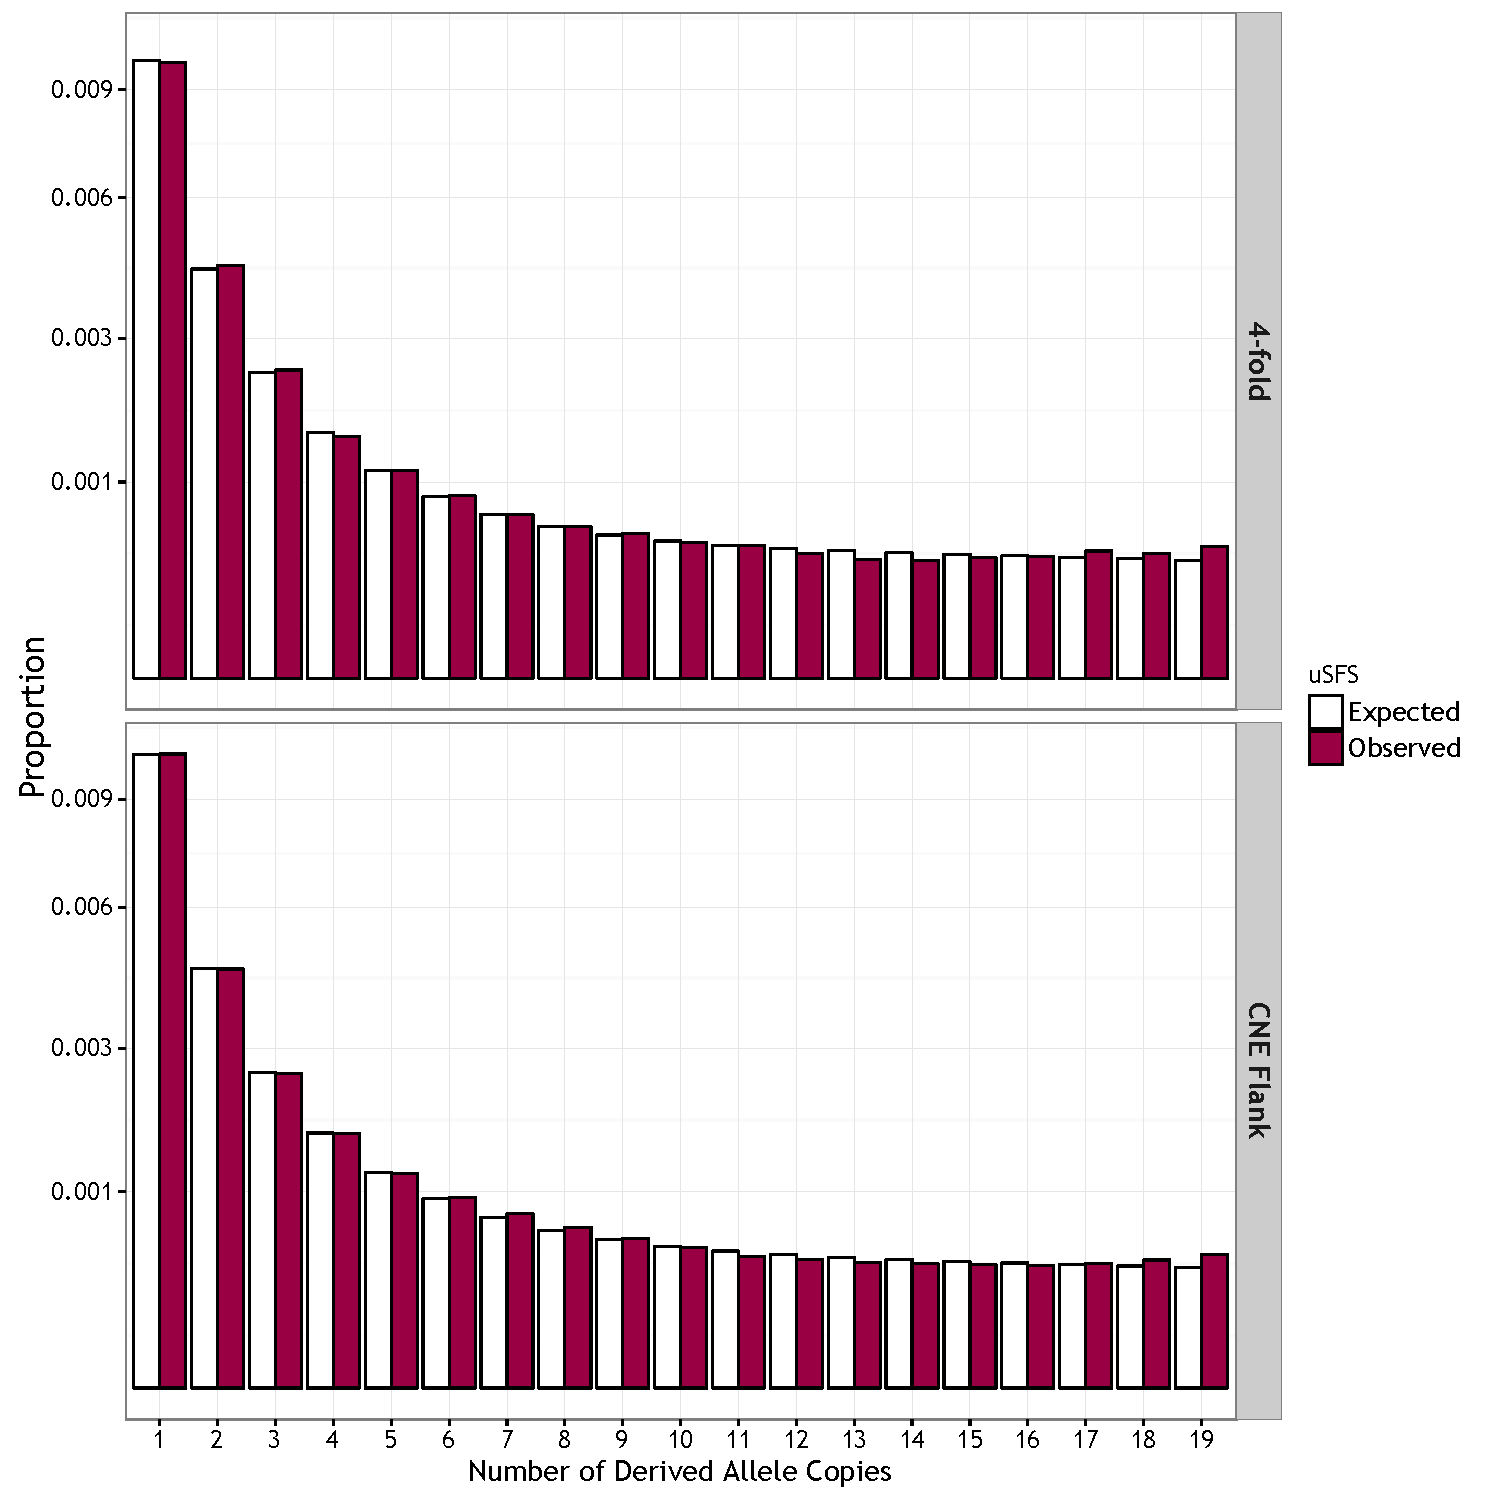
\includegraphics[width=\textwidth]{/Users/s0784966/Dropbox/Thesis/chapter3Appendix/Figures/FigureS1.pdf}}
 \caption[A comparison of the uSFS expected and observed under demographic models fitted to two classes of sites]{A comparison of the uSFS expected and observed under the best-fitting demographic models for two classes of putatively neutral sites, 4-fold degenerate synonymous sites and CNE-flanking sequences.}
 \label{fig:CS1}
\end{figure}



 \begin{figure}[h!]
   \centering      
   \noindent\makebox[\textwidth]{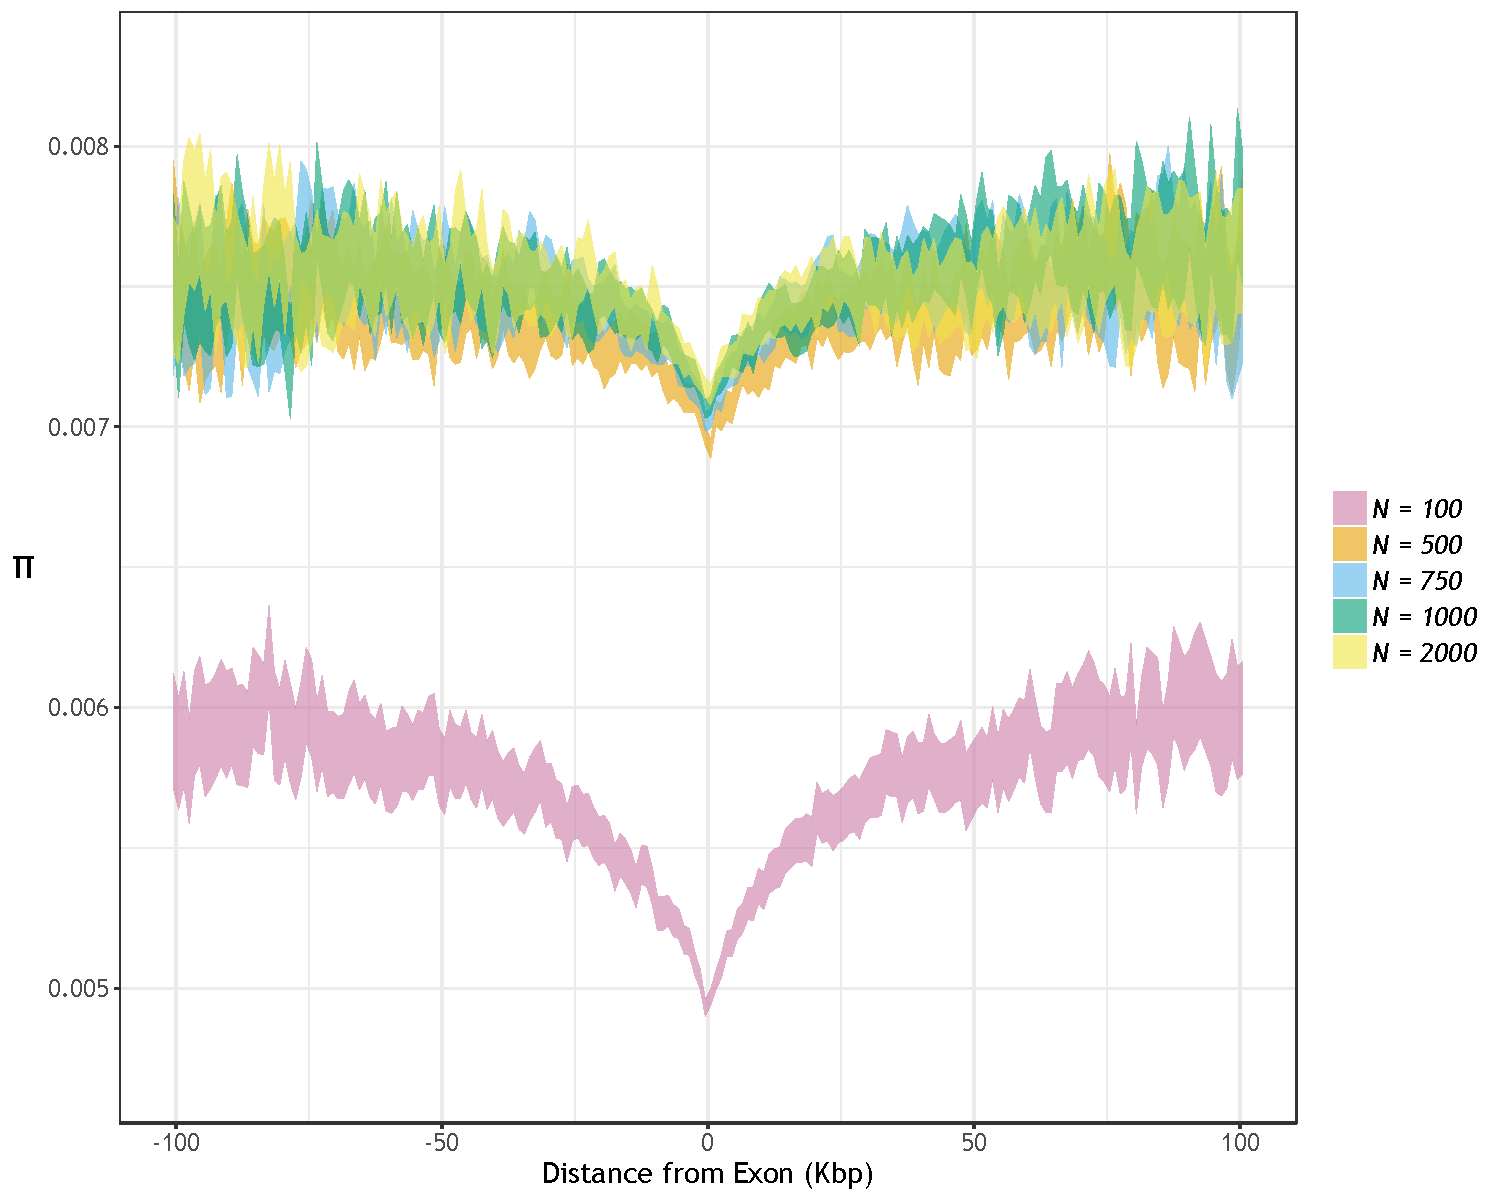
\includegraphics[width=\textwidth]{/Users/s0784966/Dropbox/Thesis/chapter3Appendix/Figures/FigureS2.pdf}}
 \caption[The effect of population size on patterns of diversity obtained from simulated populations]{The effect of population size on patterns of diversity obtained from simulated populations. }
 \label{fig:CS2}
\end{figure}



 \begin{figure}[h!]
   \centering      
   \noindent\makebox[\textwidth]{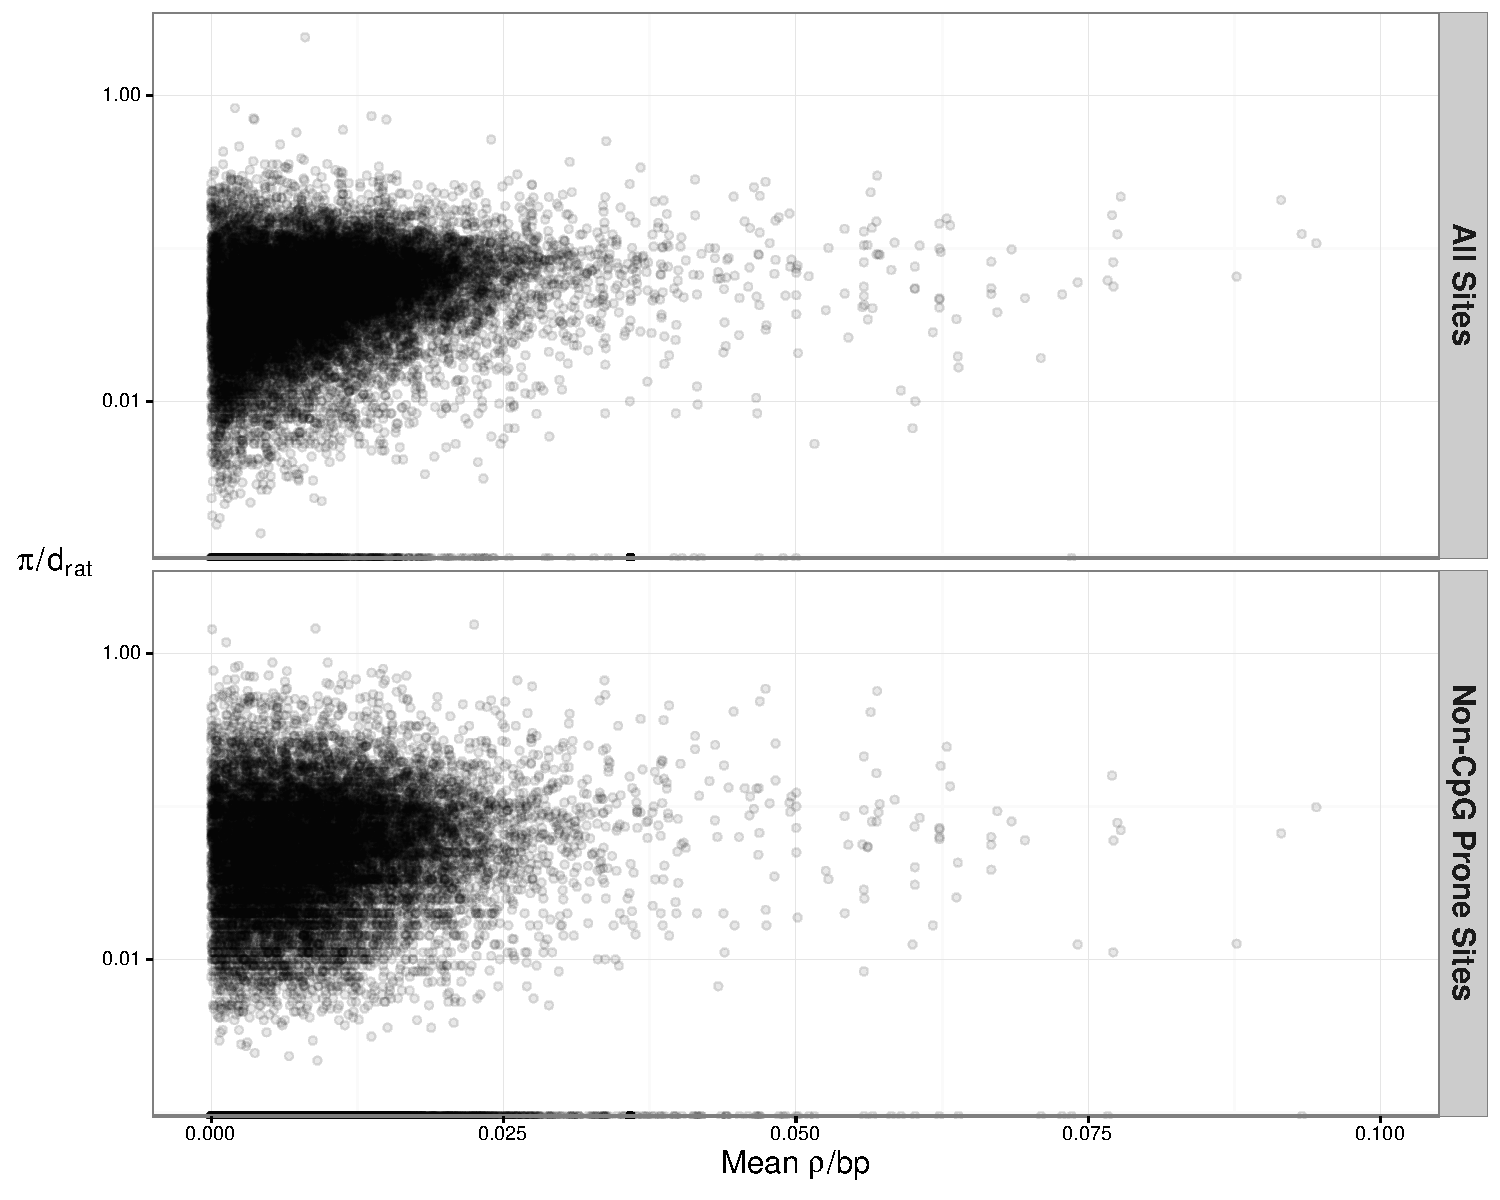
\includegraphics[width=\textwidth]{/Users/s0784966/Dropbox/Thesis/chapter3Appendix/Figures/FigureS3.pdf}}
 \caption[Estimates of unscaled $\pi$ around protein-coding exons and CNEs in \textit{M. m. castaneus} compared to the values observed in simulated populations - physical distance]{Estimates of unscaled $\pi$ around protein-coding exons and CNEs in \textit{M. m. castaneus} (black line) compared to the values observed in simulated populations (coloured ribbons) when distances are measured using physical distances.}
 \label{fig:CS3}
\end{figure}



 \begin{figure}[h!]
   \centering      
   \noindent\makebox[\textwidth]{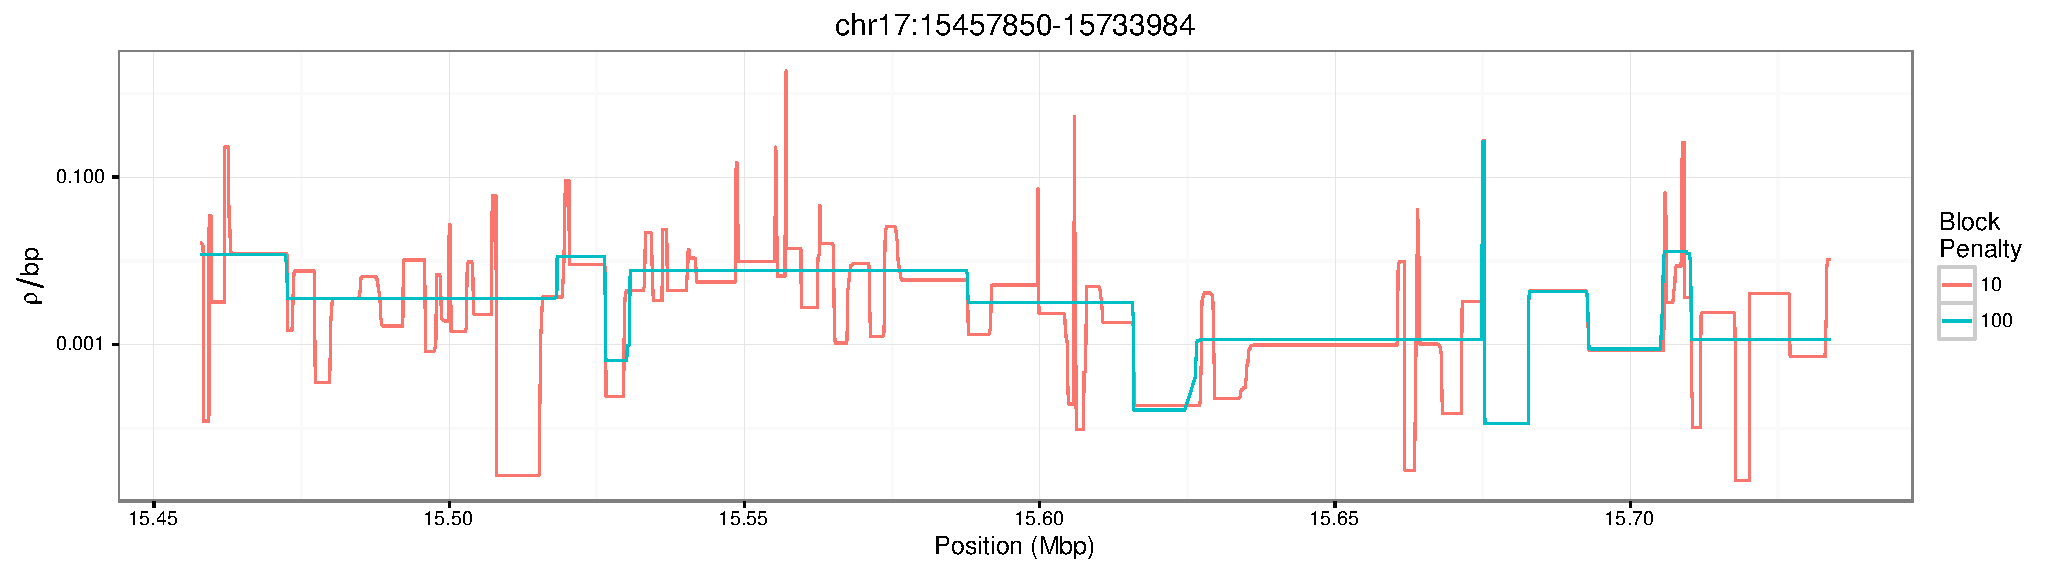
\includegraphics[width=\textwidth]{/Users/s0784966/Dropbox/Thesis/chapter3Appendix/Figures/FigureS4.pdf}}
 \caption[Estimates of unscaled $\pi$ around protein-coding exons and CNEs in \textit{M. m. castaneus} compared to the values observed in simulated populations - genetic distance]{Estimates of unscaled $\pi$ around conserved non-coding elements in \textit{M. m. castaneus} (black line) compared to the values observed in simulated populations (coloured ribbons) when distances are measured using population-scale genetic distances.}
 \label{fig:CS4}
\end{figure}



 \begin{figure}[h!]
   \centering      
   \noindent\makebox[\textwidth]{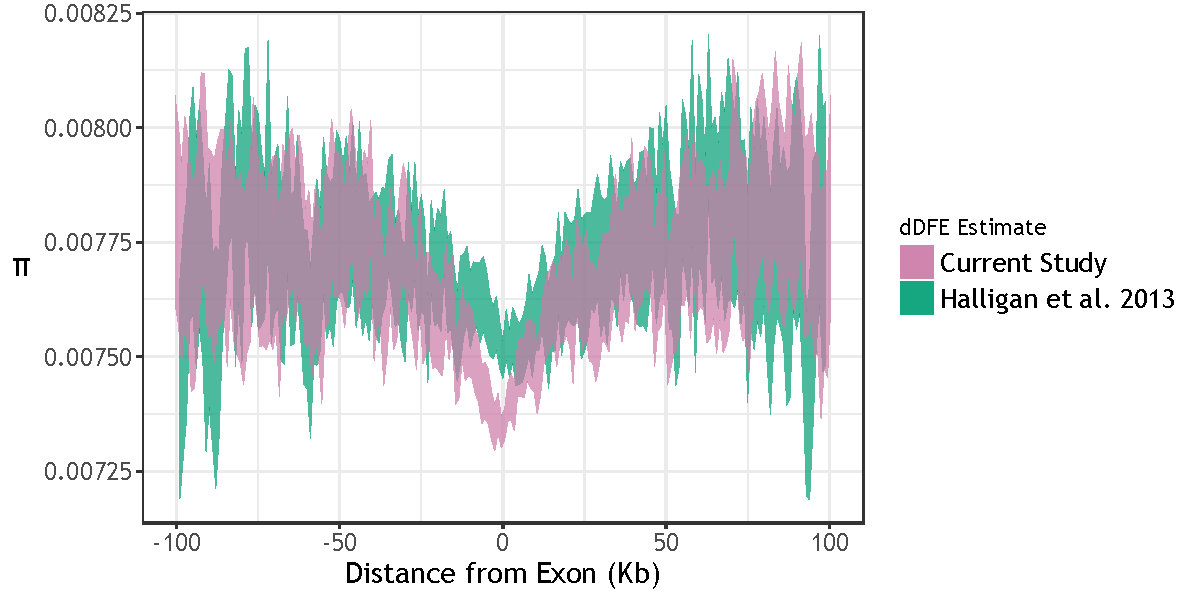
\includegraphics[width=\textwidth]{/Users/s0784966/Dropbox/Thesis/chapter3Appendix/Figures/FigureS5.pdf}}
 \caption[Comparison of nucleotide diversity ($\pi$) around protein-coding exons in simulated populations assuming a discrete or a continuous model of the dDFE]{Comparison of nucleotide diversity ($\pi$) around protein-coding exons in simulated populations under either the discrete-class dDFE estimated in the current study or the gamma dDFE estimated by \cite{RN122}}
 \label{fig:CS5}
\end{figure}



 \begin{figure}[h!]
   \centering      
   \noindent\makebox[\textwidth]{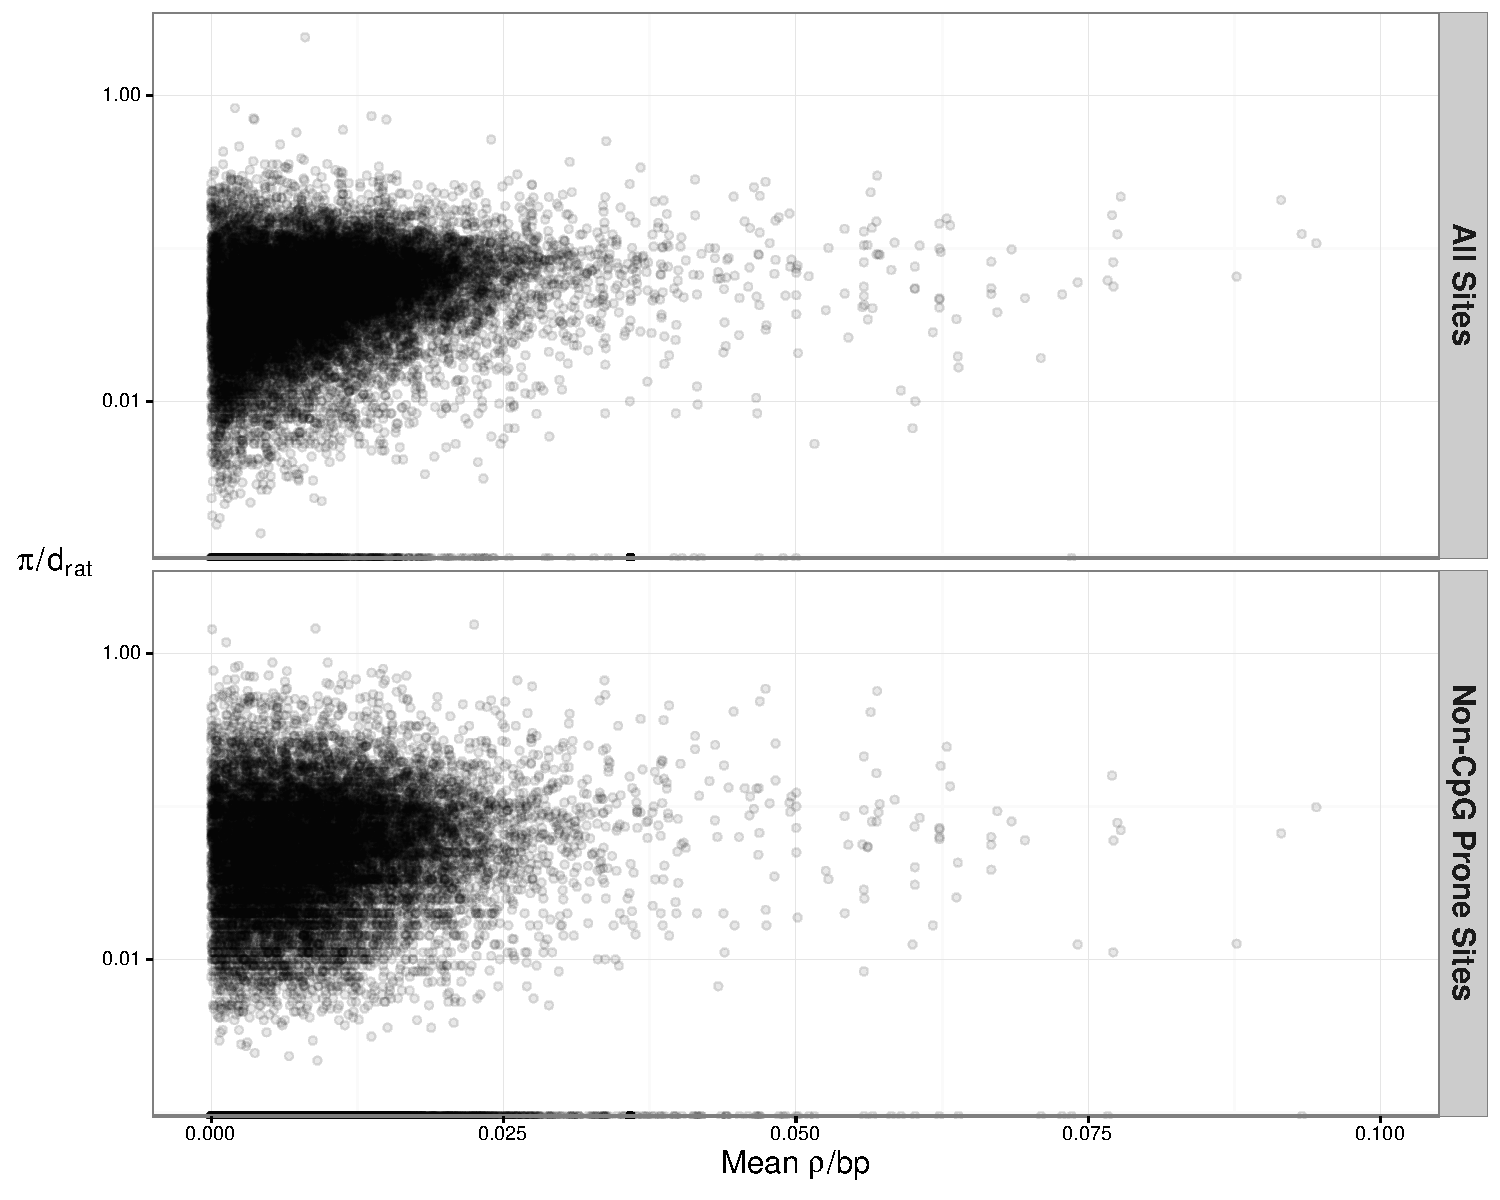
\includegraphics[width=\textwidth]{/Users/s0784966/Dropbox/Thesis/chapter3Appendix/Figures/FigureS6.pdf}}
 \caption[The demographic correction and uSFS for 4-fold sites in \textit{M. m. castaneus} and synonymous sites simulated under Model A or Model B selection parameters]{The demographic correction and uSFS for 4-fold sites in \textit{M. m. castaneus} and synonymous sites simulated under Model A or Model B selection parameters. The upper panel shows the proportional deviation between the observed uSFS and that expected under the best-fitting demographic model. The lower panel shows the uSFS.}
 \label{fig:CS6}
\end{figure}



 \begin{figure}[h!]
   \centering      
   \noindent\makebox[\textwidth]{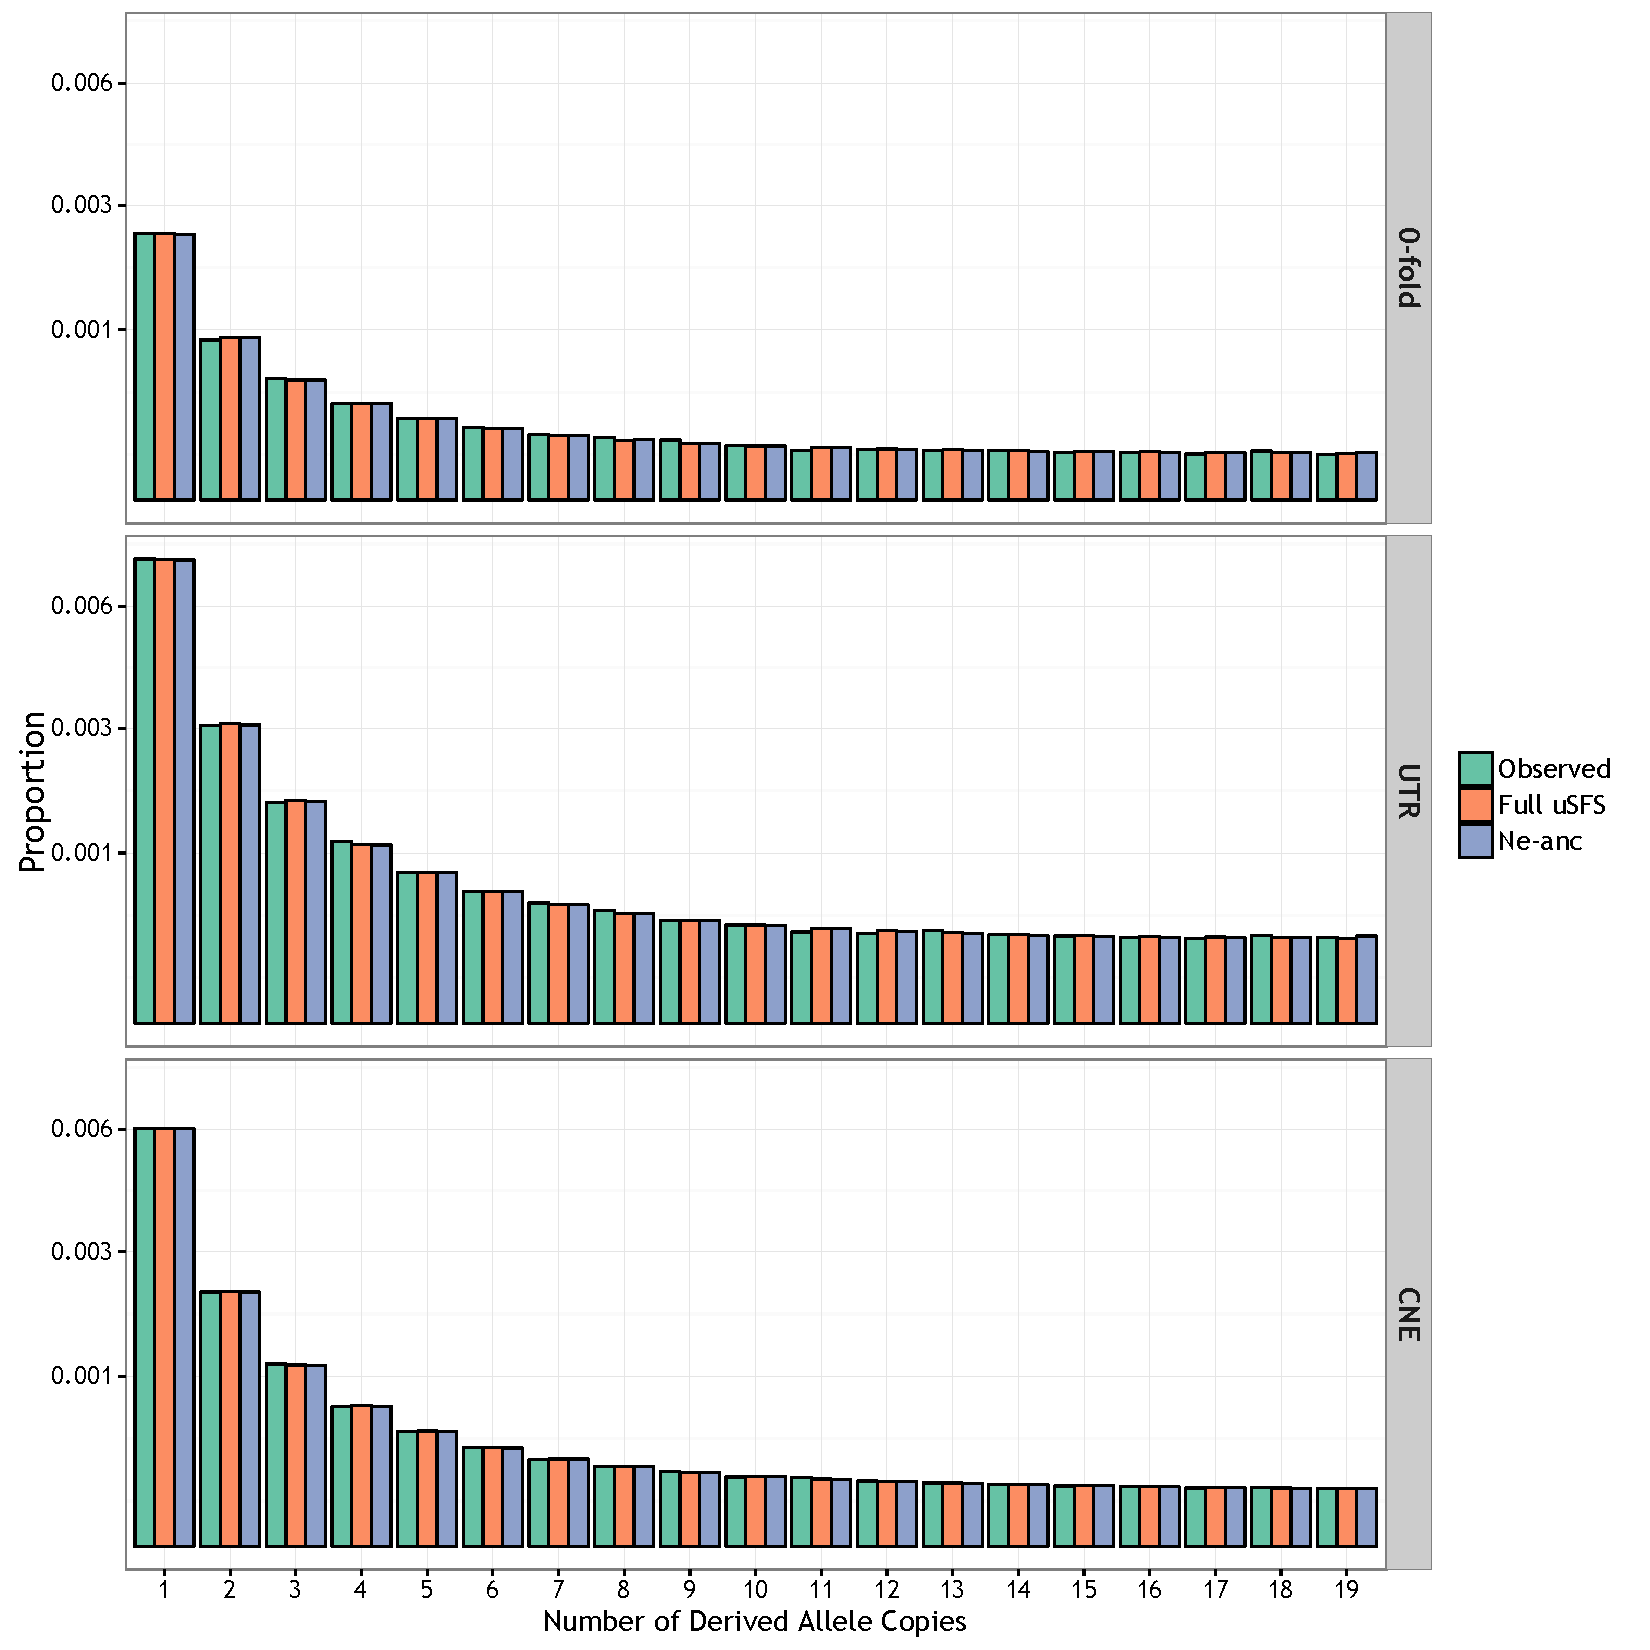
\includegraphics[width=\textwidth]{/Users/s0784966/Dropbox/Thesis/chapter3Appendix/Figures/FigureS7.pdf}}
 \caption[A comparison of the observed uSFS  with that expected under the best-fitting selection models for three classes of functional sites]{A comparison of the observed uSFS  with that expected under the best-fitting selection models for three classes of functional sites. }
 \label{fig:CS7}
\end{figure}



 \begin{figure}[h!]
   \centering      
   \noindent\makebox[\textwidth]{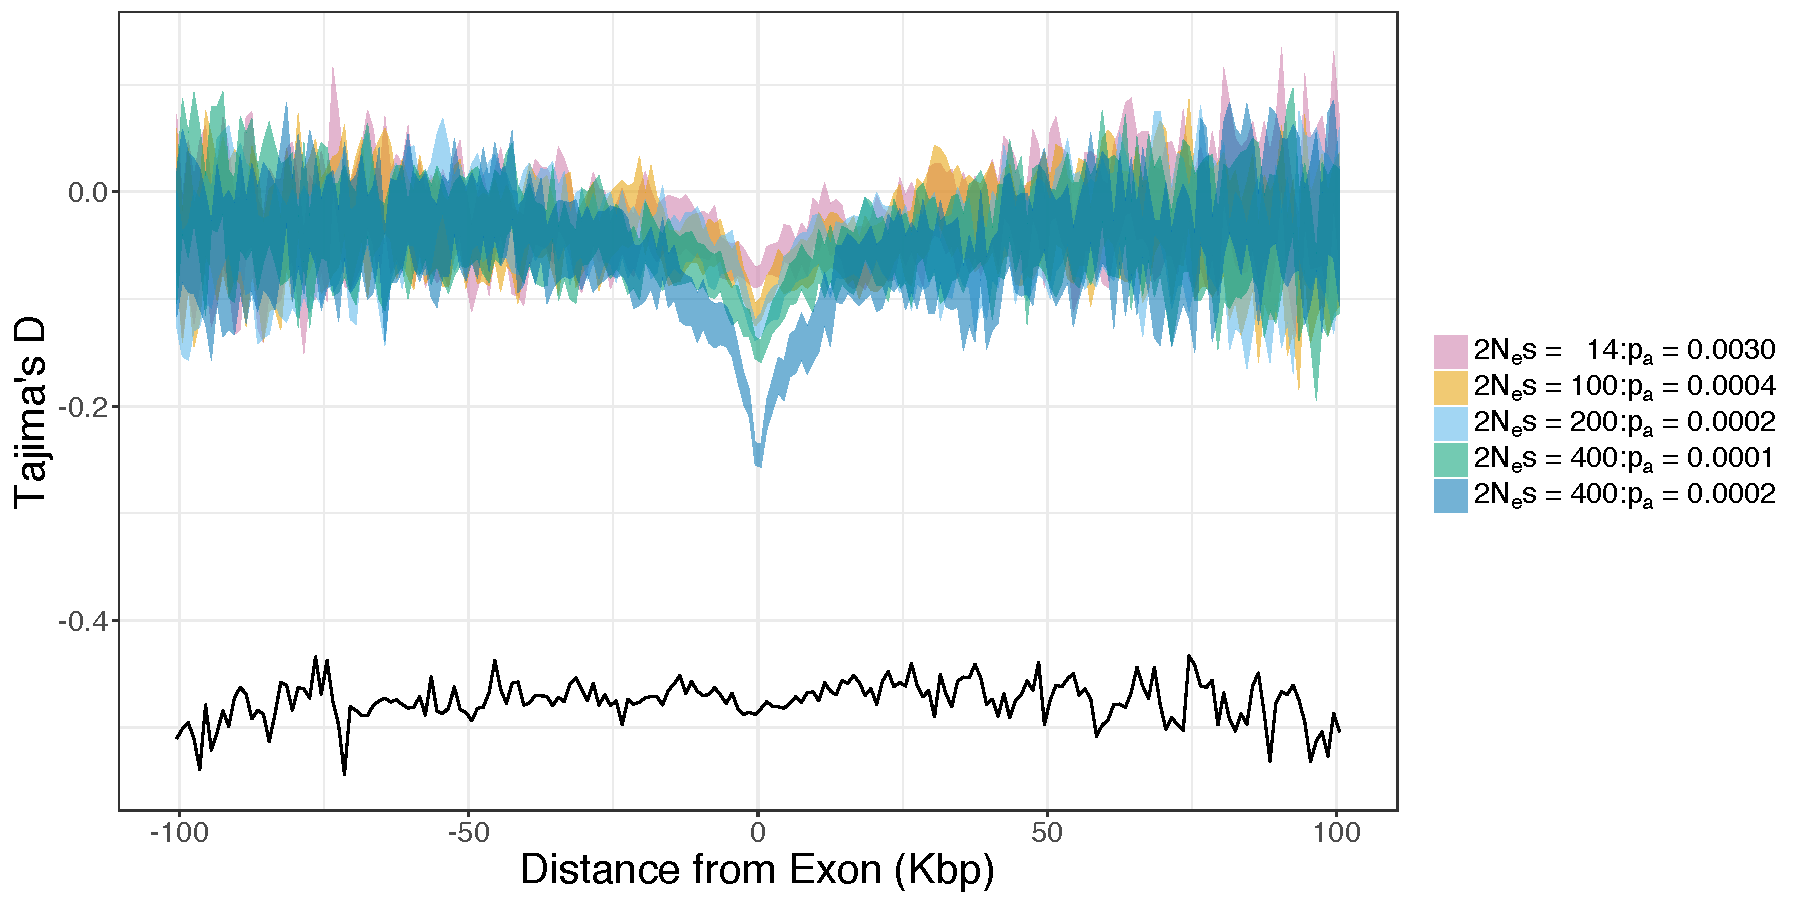
\includegraphics[width=\textwidth]{/Users/s0784966/Dropbox/Thesis/chapter3Appendix/Figures/FigureS8.pdf}}
 \caption[The pattern of Tajima’s \textit{D} around protein-coding exons for simulations assuming strongly selected advantageous mutations]{The pattern of Tajima’s \textit{D} around protein-coding exons for simulations assuming strongly selected advantageous mutations.}
 \label{fig:CS8}
\end{figure}
